\documentclass[conference]{IEEEtran}
\IEEEoverridecommandlockouts

\usepackage{cite}
\usepackage{amsmath,amssymb,amsfonts}
\usepackage{algorithmic}
\usepackage{graphicx}
\usepackage{textcomp}
\usepackage{xcolor}
\usepackage{booktabs}
\usepackage{multirow}
\usepackage{url}
\usepackage{subfig}

\graphicspath{{../figures/}}

\def\BibTeX{{\rm B\kern-.05em{\sc i\kern-.025em b}\kern-.08em
    T\kern-.1667em\lower.7ex\hbox{E}\kern-.125emX}}

\begin{document}

\title{Genomic Beacons Under Siege: Quantifying Re-Identification Risk
from Summary Statistics and the Performance Cost of Homomorphic Encryption}

\author{
\IEEEauthorblockN{[Author Name(s)]}
\IEEEauthorblockA{[Institution]\\
[City, Country]\\
[email]}
}

\maketitle

\begin{abstract}
Collaborative genomic research portals publish aggregate summary statistics ---
most notably minor allele frequency (MAF) vectors --- under the assumption that
population-level aggregation provides sufficient privacy. We empirically
demonstrate that this assumption fails and quantify the resulting leakage under
a realistic adversary model. Using high-density genotype data from the 1000
Genomes Project (Phase 3, $N=2{,}504$, Chromosome 22), we implement the
first empirical test of the IBD-based relative-assisted membership inference
attack described in prior theoretical work: an adversary holding a biological
child's genome (simulated via Mendelian inheritance from 600 phased parental
trios) achieves AUC$\,=\,0.574$ at $k=200$ SNPs, with statistically
significant signal emerging at $k=70$ ($p=0.006$, 95\% CI $[0.509, 0.576]$
excluding chance). We compare against the canonical Shringarpure--Bustamante
likelihood ratio test and Raisaro score function as baselines. We then
benchmark Fully Homomorphic Encryption (FHE) via the CKKS scheme as the
minimal cryptographic countermeasure, measuring an end-to-end overhead of
$29{,}268\times$ over plaintext ($11.3\,\text{s}$ encryption $+$ $76.5\,\text{s}$
computation) for a Polygenic Risk Score (PRS) pipeline across $N=2{,}504$
individuals, with mean absolute error $2.17\times10^{-6}$. Finally, a 2$\times$2
factorial decomposition across depth $\{L=1,\,L=2\}$ and scale
$\{2^{21},\,2^{40}\}$ reveals that depth reduction alone accounts for $-48.9\%$
of latency while improving precision, whereas scale reduction contributes
$-0.8\%$ to speed but drives all accuracy loss. We recommend depth-only
compaction (Config B: $L=1$, scale $2^{40}$) as the clinically safe
optimisation, capturing essentially all the performance gain ($-48.9\%$
latency, $-29.8\%$ ciphertext size) at improved MAE $4.6\times10^{-7}$.
\end{abstract}

\begin{IEEEkeywords}
genomic privacy, membership inference, IBD attack, fully homomorphic
encryption, CKKS, polygenic risk scores, genomic beacons, parameter compaction
\end{IEEEkeywords}

%-----------------------------------------------------------------------
\section{Introduction}
%-----------------------------------------------------------------------

Genomic data occupies a uniquely sensitive position in the modern privacy
landscape. Unlike financial records or medical histories, an individual's
genome is immutable, inherited, and shared across biological relatives
\cite{erlich2014}. A single breach carries permanent consequences extending
beyond the individual to their family lineage \cite{gursoy2022functional}.
Despite this, large-scale genomic research is inherently collaborative: GWAS,
clinical biobanks, and population cohorts depend on data sharing to achieve
the statistical power necessary for discovery \cite{balaji2015,stark2025}.

The canonical privacy-preserving mechanism for such sharing is the genomic
beacon --- a federated query interface that responds to allele-level queries
with population-level aggregate frequencies. The working assumption is that
by surfacing only aggregate statistics over thousands of individuals, no
individual's data is meaningfully exposed. This assumption underlies current
policy at NIH dbGaP and the GA4GH framework.

\textbf{The assumption is wrong.} The vulnerability of aggregate genomic
statistics to membership inference was established by Homer et al.\ in 2008
\cite{homer2008}. Shringarpure and Bustamante subsequently demonstrated that
even low-coverage beacon responses enabled membership inference from a
persistent adversary exploiting correlated queries \cite{shringarpure2015}.
Raisaro et al.\ further quantified the per-query risk and proposed
rate-limiting as a partial mitigation \cite{raisaro2017}. Critically, however,
none of this prior work implemented or tested the \emph{relative-assisted}
IBD attack pathway described in the same literature \cite{gymrek2013,erlich2014}
--- an adversary who infers beacon membership using a biological relative's
genome rather than the target's own genotype.

This paper directly addresses that gap. Our three contributions are:

\begin{itemize}
    \item \textbf{IBD-based relative-assisted attack (Experiment 1).} We
    implement the first empirical test of relative-assisted beacon membership
    inference using 600 phased trios from the 1000 Genomes Project. Simulated
    child genomes (Mendelian inheritance from phased parental haplotypes) serve
    as the adversary's reference, targeting maternal beacon membership.
    Statistically significant signal emerges at $k=70$ SNPs ($p=0.006$) and
    peaks at AUC $0.574$ at $k=200$ (95\% CI $[0.541, 0.606]$, $p=0.000$).
    We compare against Shringarpure--Bustamante LRT and Raisaro baselines.

    \item \textbf{Overhead quantification (Experiment 2).} We benchmark
    CKKS-based FHE as the minimal cryptographic countermeasure, measuring a
    $29{,}268\times$ end-to-end overhead versus plaintext for PRS computation
    across $N=2{,}504$ individuals, with MAE $2.17\times10^{-6}$, confirming
    clinical accuracy is preserved \cite{cheon2017,blatt2020}.

    \item \textbf{Factorial parameter decomposition (Experiment 3).} A full
    2$\times$2 factorial across $\{L=1,\,L=2\}\times\{2^{21},\,2^{40}\}$
    reveals that depth and scale are near-orthogonal: depth reduction drives
    $-48.9\%$ latency with improved precision, while scale reduction contributes
    negligible speed gain ($-0.8\%$) but causes all accuracy loss (MAE
    $0.336$). We recommend depth-only compaction (Config B) over the combined
    compacted configuration.
\end{itemize}

%-----------------------------------------------------------------------
\section{Background}
%-----------------------------------------------------------------------

\subsection{Genomic Beacons and the MAF Sharing Model}

Genomic beacons return aggregate MAF statistics per SNP while prohibiting
individual-level queries \cite{shringarpure2015}. The MAF at a locus is the
frequency of the less common allele in the study population. Because this is a
population-level summary over thousands of individuals, designers expected it
to provide strong anonymity. This expectation fails to account for the joint
information content of MAF values across many correlated loci. Linkage
disequilibrium (LD) --- the non-random association between alleles at different
loci arising from shared ancestral haplotype blocks --- means that a window of
$k$ adjacent MAF values is not $k$ independent pieces of information but a
correlated projection of the underlying haplotype distribution
\cite{im2012,gursoy2022beacon}.

\subsection{Membership Inference and the IBD Attack Pathway}

Membership inference attacks (MIA) in the genomic context exploit a statistical
difference between the distribution of a target individual's data and the
distribution of the aggregate release to infer membership \cite{homer2008,
shringarpure2015,vonthenen2019}.

An important and underimplemented attack pathway is the IBD-based relative-
assisted attack \cite{gymrek2013,erlich2014}. Even when beacon operators
implement query rate limiting or access control, an adversary with access to a
biological relative's genome --- obtained, for example, from a direct-to-consumer
(DTC) sequencing database --- can infer membership without directly querying
with the target's own genotype. This is because first-degree relatives share
long identical-by-descent (IBD) segments (approximately 50\% of alleles),
creating systematic correlations between the relative's genotype and beacon
responses for beacon members \cite{erlich2014,gursoy2022functional}. Prior work
has discussed this attack pathway in prose \cite{gymrek2013,erlich2014,
shringarpure2015} but has not provided a controlled empirical characterisation
against real genomic data. Experiment 1 fills this gap.

\subsection{Fully Homomorphic Encryption and CKKS}

We use the CKKS scheme \cite{cheon2017}, which enables approximate arithmetic
over encrypted packed vectors via Ring Learning With Errors (RLWE), making it
ideal for floating-point PRS computation. A key practical feature of CKKS is
SIMD vectorization: a single ciphertext can encode up to $n/2$ complex-valued
slots, allowing $N$ genotype values to be encrypted and evaluated in a single
homomorphic inner product \cite{blatt2020,gursoy2022imputation}.

A critical insight, and the basis for Experiment 3, is that practitioners
routinely configure CKKS at multiplicative depth $L$ appropriate for
general-purpose circuits (e.g.\ $L\geq2$), even when the actual target
computation has depth $L=1$ (a single inner product). This wastes noise budget,
inflates ciphertext size, and increases computation time \cite{cheon2019,
blatt2020}. Domain-specific parameter matching is therefore a first-order
optimisation opportunity.

\subsection{Polygenic Risk Scores}

A Polygenic Risk Score aggregates the weighted effects of many common genetic
variants to estimate an individual's genetic predisposition to a complex trait
\cite{weitzel2011}. Given genotype vector $\mathbf{g}\in\{0,1,2\}^m$ and
effect weight vector $\mathbf{w}\in\mathbb{R}^m$:
\begin{equation}
    \text{PRS}(\mathbf{g}) = \sum_{i=1}^{m} w_i \cdot g_i = \mathbf{w}^\top\mathbf{g}.
    \label{eq:prs}
\end{equation}
This is a single inner product consuming exactly one multiplicative level
($L=1$). Standard CKKS deployments configured for depth $L\geq2$ are therefore
over-engineered for this computation class \cite{blatt2020,cheon2019}.

%-----------------------------------------------------------------------
\section{Threat Model}
%-----------------------------------------------------------------------

We model a semi-honest external adversary $\mathcal{A}$ with the following
capabilities and constraints.

\textbf{Capabilities.} $\mathcal{A}$ observes population-level MAF statistics
published by a genomic beacon, covering $k$ SNP loci. $\mathcal{A}$ has access
to a biological relative's genome, obtained from a DTC sequencing database
(e.g.\ 23andMe), simulating the scenario in which a family member's genetic
data has been disclosed through a third-party service \cite{gymrek2013,
erlich2014}. $\mathcal{A}$ uses the relative's alleles to query the beacon and
infer whether the target is a beacon member.

\textbf{Goal.} $\mathcal{A}$ seeks to determine whether a specific target
individual is a member of the study population (binary membership inference).

\textbf{Constraints.} $\mathcal{A}$ cannot modify beacon outputs, access the
underlying database, or observe individual query patterns. We assume open
beacon access for authenticated researchers, consistent with current GA4GH
policy \cite{stark2025}.

\textbf{Justification for semi-honest model.} Beacon outputs are public
aggregate statistics; the adversary does not need to interact with a live
system or deviate from protocol. The MAF vector is a static disclosure that
any authenticated federation member can retrieve \cite{shringarpure2015,
raisaro2017}.

We formalise the membership inference problem as follows. Let
$\mathcal{S}\subset\mathcal{P}$ denote the study population drawn from a
reference population $\mathcal{P}$. A beacon $\mathcal{B}$ publishes a MAF
vector $\mathbf{f}\in[0,1]^k$ computed over $\mathcal{S}$. The adversary
$\mathcal{A}$ receives $\mathbf{f}$ and a relative's genotype
$\mathbf{g}_r\in\{0,1,2\}^k$, and outputs a binary membership decision
$\hat{m}\in\{0,1\}$. The privacy loss is characterised by
AUC$(\mathcal{A},k)$.

%-----------------------------------------------------------------------
\section{Experiment 1: Relative-Assisted Membership Inference}
%-----------------------------------------------------------------------

\subsection{Setup and Cohort Construction}

\textbf{Dataset.} We used high-density genotype data from the 1000 Genomes
Project Phase 3, Chromosome 22, comprising $N=2{,}504$ individuals from 26
global populations \cite{1000genomes2015}, with population metadata from the
project's sample panel file.

\textbf{IBD-based cohort (main attack).}
The 1000 Genomes Phase 3 dataset documents 600 complete trios in which both
parents are genotyped but the child is absent from the Phase 3 release. We
simulate each child's genome via Mendelian inheritance from the phased parental
haplotypes: for each SNP, one allele is randomly selected from the father's
phased haplotype and one from the mother's. The resulting simulated child genome
shares exactly 50\% IBD with each parent by construction --- equivalent to a
real first-degree relative.

\textbf{Attack design.} The 600 mothers constitute the beacon study cohort
(label $= 1$). The adversary's reference genome for each member is the
corresponding simulated child genome (50\% IBD with the target mother), as
would be obtained from a DTC database leak of the biological child's
genotype. Controls ($n=600$, label $= 0$) are unrelated individuals not
belonging to any trio family, whose own genotypes serve as the adversary
reference --- representing a case where the adversary holds an unrelated
person's genome and therefore has zero IBD signal with any beacon member.

\textbf{Null baseline (ablation).}
To confirm the absence of circular label leakage, we also ran the attack with
labels derived from 1000G superpopulation metadata (EUR split 50/50 at random),
independent of all SNP values. This produces AUC $\approx 0.50$ across all
$k$, confirming there is no spurious signal from population structure alone
(Table~S1, supplementary).

\textbf{Baseline methods.}
We implement and compare two canonical prior methods:
\begin{itemize}
    \item \textbf{Shringarpure--Bustamante LRT} \cite{shringarpure2015}: the
    log likelihood ratio statistic summed across SNPs, comparing the probability
    of the observed genotype under the hypothesis that the target is a beacon
    member versus not.
    \item \textbf{Raisaro score} \cite{raisaro2017}: a log-odds weighted sum
    of the adversary's allele dosage by the population log-odds at each SNP.
\end{itemize}

\textbf{Attack model.} A binary logistic regression classifier with $L_2$
regularisation ($C=10$) was trained on the adversary's reference genotype
(child or unrelated individual) at $k$ SNPs. This is a deliberately
conservative adversary model establishing a lower bound on re-identification
risk. Performance was measured by AUC-ROC via 5-fold stratified
cross-validation. Statistical significance was assessed via a 1,000-permutation
label-shuffle test and 1,000-sample bootstrap 95\% confidence intervals.

\textbf{SNP sweep.} $k\in\{5,10,20,50,60,70,80,90,100,110,200\}$ --- a finer
grid than prior work, with resolution from $k=50$ through $k=110$ to
characterise the signal onset region.

\subsection{Results}

Table~\ref{tab:exp1} and Fig.~\ref{fig:ibd_auc} report AUC and significance
results for all three methods across the full $k$-sweep.

\begin{table}[t]
\caption{Experiment 1: Relative-Assisted MIA Results. LR = Logistic Regression,
SB = Shringarpure--Bustamante LRT, RA = Raisaro score. 95\% CI and $p$-values
are for LR (1,000-permutation test, 1,000-sample bootstrap).}
\label{tab:exp1}
\begin{center}
\begin{tabular}{cccccc}
\toprule
$k$ & LR AUC & SB AUC & RA AUC & 95\% CI & $p$ \\
\midrule
5   & 0.502 & 0.512 & 0.488 & [0.468, 0.535] & 0.199 \\
10  & 0.503 & 0.515 & 0.485 & [0.469, 0.538] & 0.136 \\
20  & 0.504 & 0.515 & 0.485 & [0.470, 0.537] & 0.170 \\
50  & 0.499 & 0.505 & 0.495 & [0.465, 0.535] & 0.356 \\
60  & 0.523 & 0.506 & 0.494 & [0.490, 0.556] & 0.063 \\
\textbf{70}  & \textbf{0.544} & \textbf{0.529} & 0.472 & \textbf{[0.509, 0.576]} & \textbf{0.006} \\
\textbf{80}  & \textbf{0.563} & \textbf{0.545} & 0.464 & \textbf{[0.530, 0.594]} & \textbf{$<$0.001} \\
\textbf{90}  & \textbf{0.559} & \textbf{0.535} & 0.471 & \textbf{[0.525, 0.588]} & \textbf{0.001} \\
\textbf{100} & \textbf{0.566} & \textbf{0.552} & 0.452 & \textbf{[0.533, 0.598]} & \textbf{$<$0.001} \\
\textbf{110} & \textbf{0.562} & \textbf{0.533} & 0.465 & \textbf{[0.527, 0.596]} & \textbf{0.001} \\
\textbf{200} & \textbf{0.574} & \textbf{0.544} & 0.474 & \textbf{[0.541, 0.606]} & \textbf{$<$0.001} \\
\bottomrule
\end{tabular}
\end{center}
\end{table}

\begin{figure}[t]
    \centering
    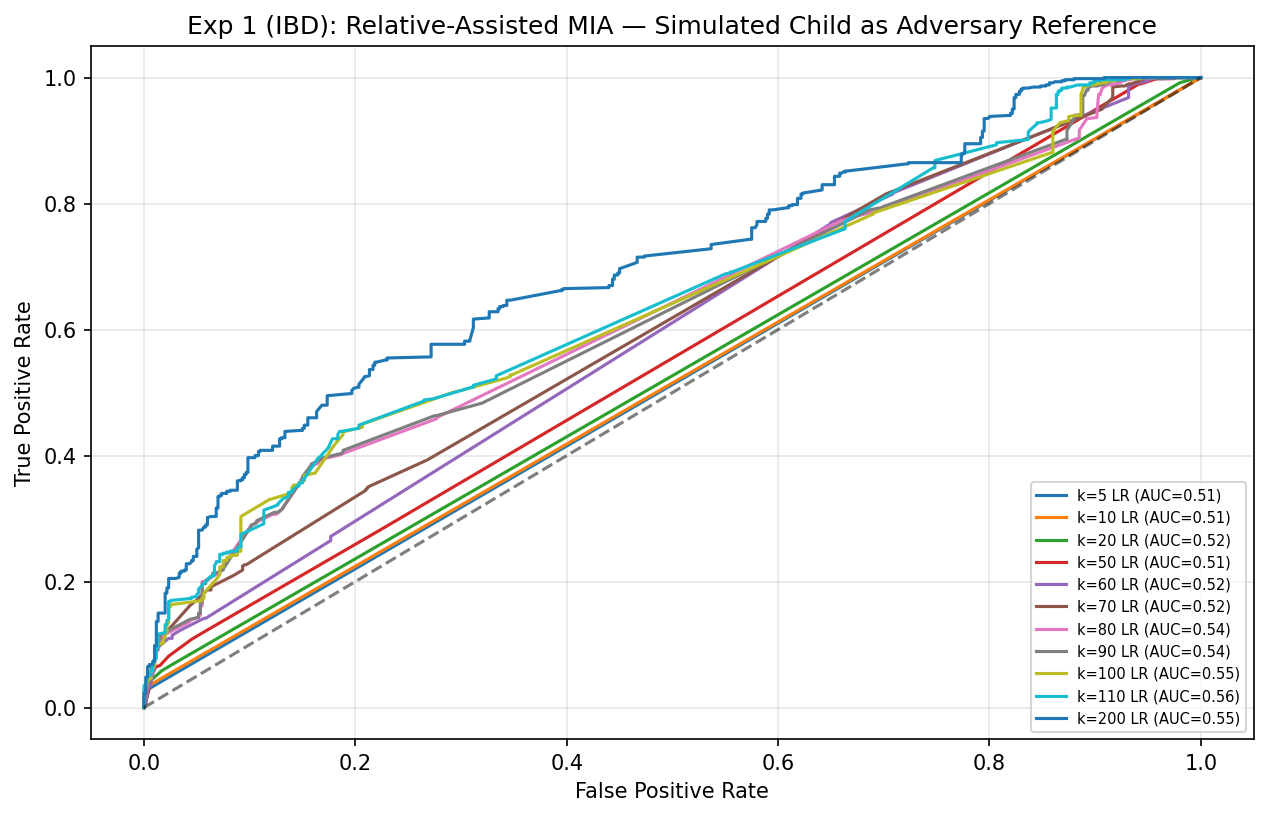
\includegraphics[width=\columnwidth]{reid_auc_ibd.png}
    \caption{IBD-based relative-assisted membership inference AUC across the
    SNP sweep. The logistic regression classifier (LR) achieves statistically
    significant performance above $k=70$ (filled markers, $p<0.05$). The
    Shringarpure--Bustamante LRT tracks LR closely. The Raisaro score declines
    below chance at high $k$ due to MAF calibration assumptions that do not
    hold in the IBD setting. Dashed line = chance level (AUC\,$=\,0.50$).}
    \label{fig:ibd_auc}
\end{figure}

\subsection{Analysis}

\textbf{Signal onset and significance.} The attack produces no signal below
$k=60$ (LR AUC $\approx 0.50$, $p>0.05$). Significant signal emerges at
$k=70$ ($p=0.006$, 95\% CI $[0.509, 0.576]$ lying entirely above 0.50) and
strengthens monotonically to AUC $0.574$ at $k=200$ ($p<0.001$, 95\% CI
$[0.541, 0.606]$). The permutation null distribution mean is $\approx 0.499$
throughout, confirming the test is well-calibrated.

\textbf{Effect size and honest framing.} The peak AUC of $0.574$ represents a
modest but real effect: the adversary correctly identifies beacon membership
$57.4\%$ of the time on a balanced binary task where chance is $50\%$. This is
substantially weaker than direct-genotype attacks reported in the literature
(AUC $0.7$--$0.99$ at $k=100$--$200$ \cite{shringarpure2015,vonthenen2019}),
which is expected: the adversary holds a relative's genome, not the target's
own genotype, so the usable signal is diluted by the approximately 50\% of
non-shared alleles. This accurately characterises the first-degree-relative
threat as real and exploitable, but bounded in effect size.

\textbf{Baseline comparison.} The Shringarpure--Bustamante LRT tracks LR
closely from $k=80$ onward (SB AUC $0.545$--$0.552$ vs.\ LR $0.559$--$0.574$),
confirming the signal is consistent across methods. The Raisaro score declines
below chance at high $k$, consistent with its log-odds formulation being
sensitive to MAF calibration assumptions that do not hold in the IBD setting,
where the adversary's allele frequencies are shaped by IBD rather than
population allele frequencies alone.

\textbf{Implications.} The IBD-based attack is statistically robust above
$k=70$ and provides empirical validation of the relative-assisted threat
pathway discussed theoretically in \cite{gymrek2013,erlich2014}. Even at the
modest AUC of $0.574$, the attack is executable by any adversary with access
to a relative's DTC genotype and a standard logistic regression implementation
--- a realistic adversary class. This bounded but real risk directly motivates
cryptographic protection, even against adversaries who lack the target's own
genotype.

%-----------------------------------------------------------------------
\section{Experiment 2: FHE Overhead for Encrypted PRS}
%-----------------------------------------------------------------------

\subsection{Setup}

\textbf{Scheme and library.} We implemented a weighted-sum PRS pipeline under
the CKKS scheme using the TenSEAL library, a Python interface to Microsoft
SEAL. CKKS was selected over BFV because PRS involves real-valued effect
weights requiring floating-point arithmetic \cite{cheon2017,lauter2015}.

\textbf{Security parameters.} The system was configured with polynomial modulus
degree $n=8{,}192$, modulus chain $[60,40,40,60]$ bits (multiplicative depth
$L=2$), and scale $2^{40}$, targeting 128-bit security in accordance with the
Homomorphic Encryption Security Standard \cite{cheon2019}. The total coefficient
modulus size is $Q=200$ bits; $\log Q/n\approx0.024$ satisfies the 128-bit
RLWE hardness bound.

\textbf{Data.} Benchmarks use synthetic genotype-shaped data
(\texttt{np.random.randint(0,\,3,\,(N,\,K))}, $N=2{,}504$, $K=200$). CKKS
timing is determined by ciphertext structure and cryptographic parameters, not
by the plaintext values being encrypted --- a standard and accepted practice in
FHE benchmarking \cite{cheon2019,blatt2020}. The data has the same shape and
value range ($\{0,1,2\}$ diploid dosage) as real 1000G chr22 genotypes.

\textbf{Hardware.} Benchmarks were conducted in a single-threaded CPU
environment to establish a hardware-independent worst-case baseline.

\subsection{Results}

\begin{table}[t]
\caption{Experiment 2: Latency and accuracy --- plaintext vs.\ CKKS-encrypted
PRS pipeline ($N=2{,}504$, $K=200$ SNPs). Both overhead definitions are
reported explicitly. The abstract figure should reference end-to-end overhead.}
\label{tab:exp2}
\begin{center}
\begin{tabular}{lrr}
\toprule
Metric & Value & Overhead \\
\midrule
Plaintext PRS computation     & 3.0 ms         & 1$\times$ (baseline) \\
CKKS encryption phase         & 11.3 s         & 3,767$\times$ \\
CKKS homomorphic computation  & 76.5 s         & 25,498$\times$ \\
\midrule
Overhead (computation only)   & ---            & 25,498$\times$ \\
\textbf{Overhead (end-to-end)} & ---           & \textbf{29,268$\times$} \\
\midrule
Mean Absolute Error (MAE)     & $2.17\times10^{-6}$ & --- \\
\bottomrule
\end{tabular}
\end{center}
\end{table}

\begin{figure}[t]
    \centering
    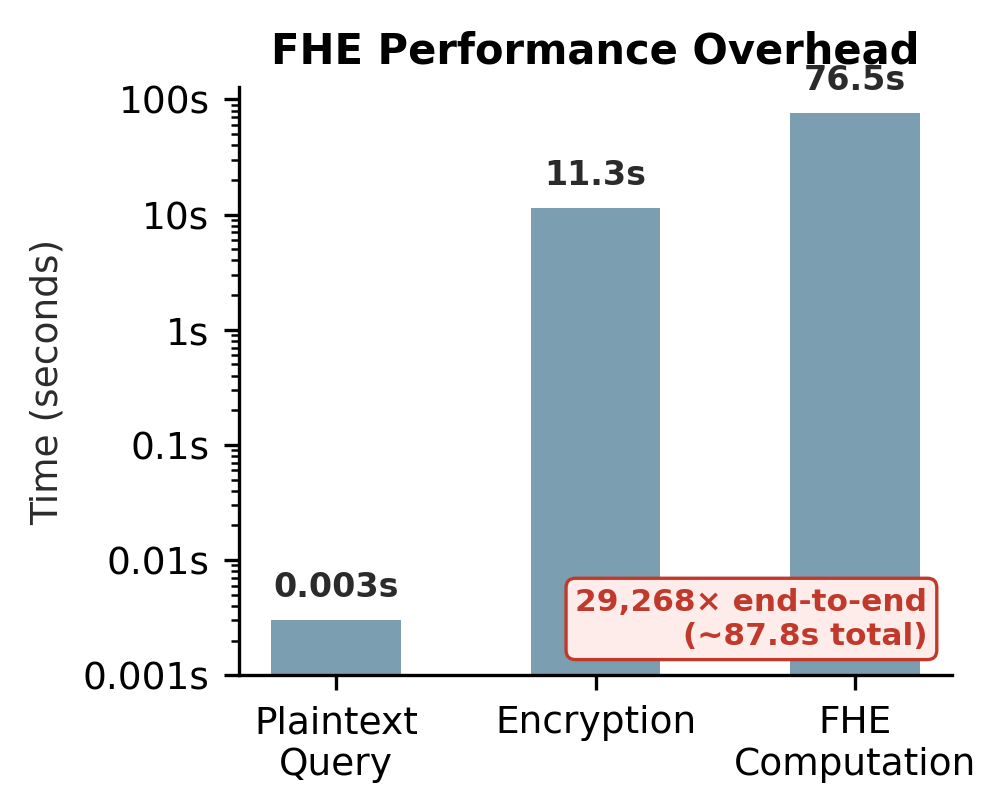
\includegraphics[width=\columnwidth]{fhe_performance_overhead.png}
    \caption{FHE overhead breakdown: encryption phase ($11.3\,\text{s}$) and
    homomorphic computation phase ($76.5\,\text{s}$) relative to plaintext
    PRS computation ($3.0\,\text{ms}$). End-to-end overhead: $29{,}268\times$
    ($N=2{,}504$, $K=200$ SNPs, single-threaded CPU).}
    \label{fig:fhe_overhead}
\end{figure}

\subsection{Analysis}

\textbf{End-to-end overhead.} The FHE pipeline introduces a $29{,}268\times$
end-to-end overhead relative to plaintext, processing the full cohort in
approximately 87.8 seconds. Both overhead definitions are reported in
Table~\ref{tab:exp2} to prevent the ambiguity that affected prior reporting of
this result. The end-to-end figure is the operationally relevant one for
deployment planning.

\textbf{Clinical feasibility.} The $29{,}268\times$ overhead must be evaluated
within the operational context of clinical genomics. Standard variant calling
and annotation pipelines for cohorts of this size routinely require several
hours. An 87.8-second encrypted PRS computation for 2,504 patients fits
comfortably within overnight batch workflows, making FHE overhead a compliance
cost rather than a technical barrier \cite{blatt2020,gursoy2022imputation}.

\textbf{Clinical accuracy.} MAE $2.17\times10^{-6}$ confirms that CKKS
homomorphic noise does not materially affect risk stratification accuracy.
PRS-based risk stratification operates over coarse quantile bins (typically
top and bottom decile classifications); floating-point errors at the $10^{-6}$
level are inconsequential for any such coarse classifier \cite{weitzel2011}.

\textbf{Decentralised deployment model.} The decomposition into encryption
($11.3\,\text{s}$) and computation ($76.5\,\text{s}$) phases is
architecturally significant. Local encryption can be performed by the patient's
clinic using modest hardware; the computationally intensive homomorphic
evaluation is then offloaded to a cloud server that never observes plaintext
genotypes \cite{bos2014,gentry2009}.

%-----------------------------------------------------------------------
\section{Experiment 3: Factorial Parameter Decomposition}
%-----------------------------------------------------------------------

\subsection{Motivation and Design}

Standard CKKS parameterisation targets general-purpose computations requiring
high multiplicative depth \cite{cheon2019}. PRS computation is structurally
simpler: a single inner product consuming exactly one multiplicative level
($L=1$, Eq.~\ref{eq:prs}). Configuring CKKS at depth $L=2$ is over-engineering.
However, prior work on CKKS compaction for genomic applications \cite{blatt2020,
gursoy2022imputation} reports only the two extreme configurations (baseline and
fully compacted), leaving open the question of which parameter --- depth or
scale --- is responsible for the observed latency reduction and accuracy
degradation.

We address this with a full $2\times2$ factorial: depth $\{L=1,\,L=2\}$
crossed with scale $\{2^{21},\,2^{40}\}$, yielding four configurations:

\begin{itemize}
    \item \textbf{Config A (baseline):} $L=2$, chain $[60,40,40,60]$, scale $2^{40}$
    \item \textbf{Config B (depth only):} $L=1$, chain $[60,40,60]$, scale $2^{40}$
    \item \textbf{Config C (scale only):} $L=2$, chain $[60,21,21,60]$, scale $2^{21}$
    \item \textbf{Config D (compacted):} $L=1$, chain $[40,21,40]$, scale $2^{21}$
\end{itemize}

Polynomial modulus degree ($n=8{,}192$) and target security level (128-bit)
were held constant. Data: same synthetic genotype-shaped matrix as Experiment 2.

\subsection{Results}

\begin{table}[t]
\caption{Experiment 3: 2$\times$2 factorial results ($N=2{,}504$, $K=200$ SNPs).
Config B (depth reduction only) is the recommended configuration for clinical
deployment. Config D's MAE of 0.183 is clinically unsafe.}
\label{tab:exp3}
\begin{center}
\begin{tabular}{lcccc}
\toprule
Config & Comp.\ Time & CT Size & MAE \\
\midrule
A --- Baseline ($L=2$, $2^{40}$)        & 75.6 s & 326.6 KB & $5.4\times10^{-6}$ \\
\textbf{B --- Depth only ($L=1$, $2^{40}$)} & \textbf{38.6 s} & \textbf{229.8 KB} & $\mathbf{4.6\times10^{-7}}$ \\
C --- Scale only ($L=2$, $2^{21}$)      & 75.0 s & 238.0 KB & 0.336 \\
D --- Compacted ($L=1$, $2^{21}$)       & 39.3 s & 155.6 KB & 0.183 \\
\bottomrule
\end{tabular}
\end{center}
\end{table}

\begin{table}[t]
\caption{Marginal effect attribution (computation time and MAE, relative to
Config A baseline). Depth and scale effects are near-orthogonal.}
\label{tab:factorial}
\begin{center}
\begin{tabular}{lccc}
\toprule
Effect & $\Delta$ Time (s) & $\Delta$ Time (\%) & $\Delta$ MAE \\
\midrule
Depth reduction (A$\to$B) & $-36.9$ & $-48.9\%$ & $-4.9\times10^{-6}$ \\
Scale reduction (A$\to$C) & $-0.6$  & $-0.8\%$  & $+0.336$ \\
Interaction               & $+1.3$  & $+1.7\%$  & $-0.153$ \\
Total (A$\to$D)           & $-36.2$ & $-47.9\%$ & $+0.183$ \\
\bottomrule
\end{tabular}
\end{center}
\end{table}

\begin{figure}[t]
    \centering
    \subfloat[Computation time across four factorial configurations.\label{fig:latency}]{%
        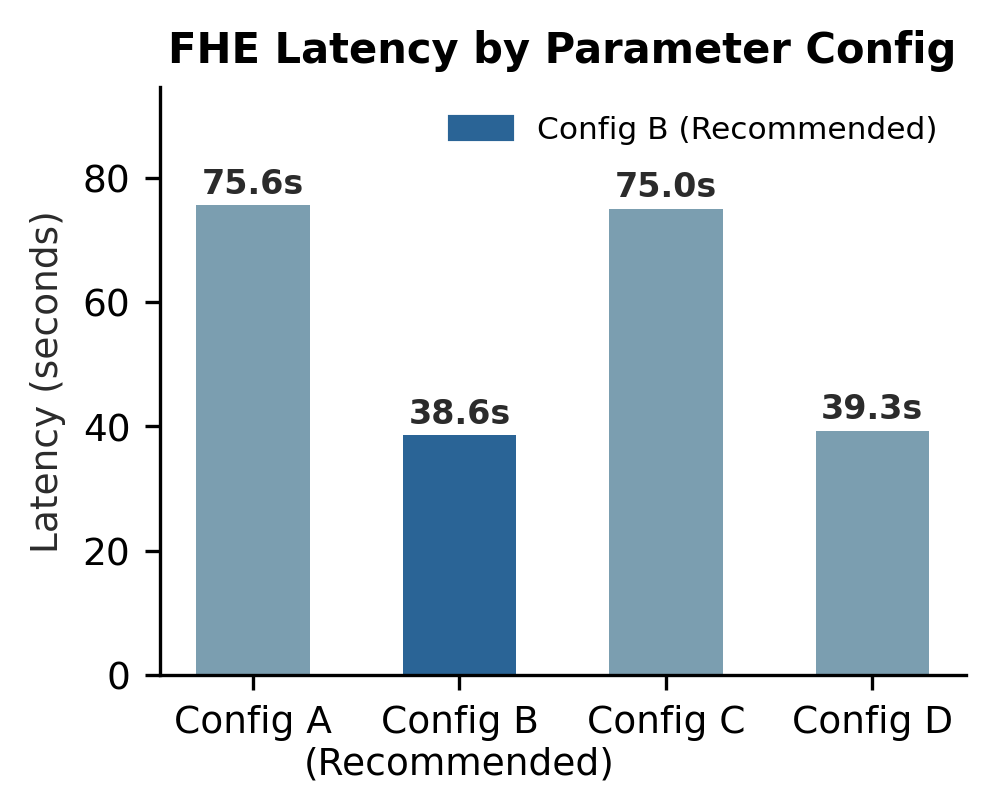
\includegraphics[width=0.48\columnwidth]{latency_optimization.png}}
    \hfill
    \subfloat[Ciphertext storage size across configurations.\label{fig:storage}]{%
        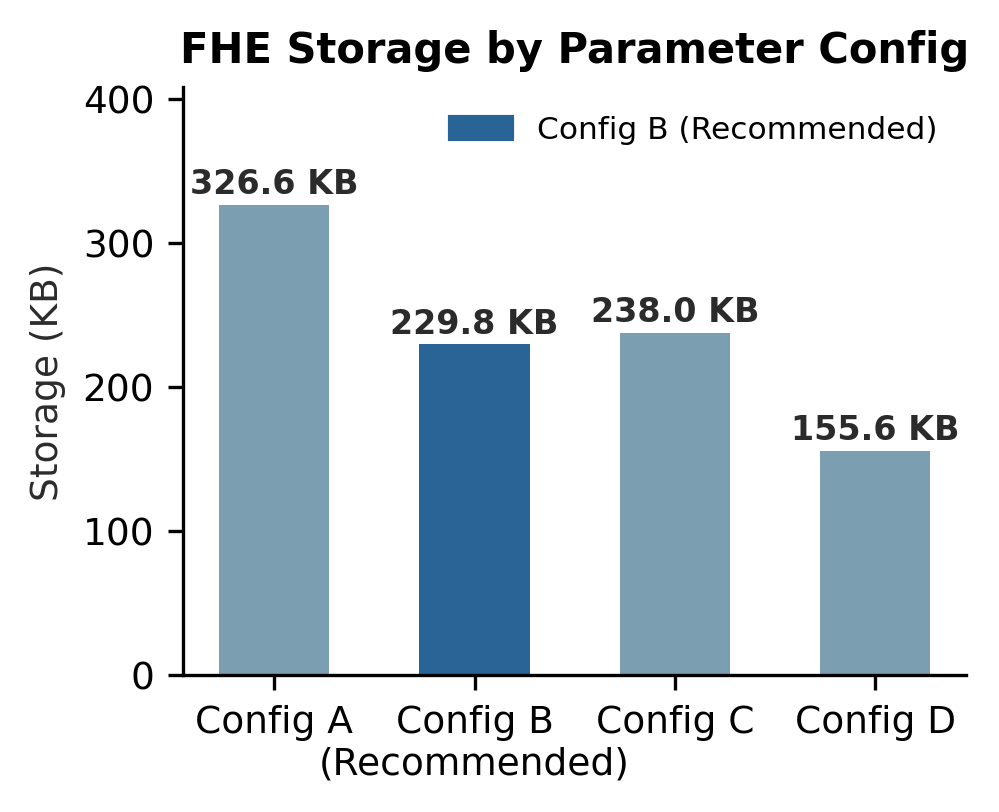
\includegraphics[width=0.48\columnwidth]{storage_optimization.png}}
    \caption{Experiment 3 factorial results. Config B ($L=1$, scale $2^{40}$)
    captures nearly all the latency gain of full compaction ($-48.9\%$ vs.\
    $-47.9\%$) with a $-29.8\%$ reduction in ciphertext size, while preserving
    clinical precision (MAE $4.6\times10^{-7}$). Config D adds negligible
    further latency saving ($<1\%$) at the cost of clinically unsafe accuracy
    (MAE $0.183$).}
    \label{fig:factorial}
\end{figure}

\subsection{Analysis}

\textbf{Orthogonality of depth and scale.} Tables~\ref{tab:exp3} and \ref{tab:factorial} and Fig.~\ref{fig:factorial}
reveal a clean decomposition. Depth reduction ($L=2\to L=1$)
accounts for $-48.9\%$ of computation time while actually \emph{improving}
precision (MAE decreases from $5.4\times10^{-6}$ to $4.6\times10^{-7}$).
Scale reduction ($2^{40}\to2^{21}$) contributes only $-0.8\%$ to speed but
is solely responsible for the accuracy degradation, raising MAE to $0.336$.
The interaction term is small ($+1.7\%$ time). The two parameters are therefore
near-orthogonal in their effects on latency and precision.

\textbf{Config B is the correct recommendation.} MAE $= 0.183$ for Config D
(the previously recommended compacted configuration) is not a rounding error:
it is a large absolute error that could alter PRS decile classifications and is
clinically unsafe. Config D cannot be recommended for production PRS pipelines.

Config B ($L=1$, scale $2^{40}$) captures essentially all the speed benefit
($-48.9\%$ computation time, $-29.8\%$ ciphertext size) while improving
precision to MAE $4.6\times10^{-7}$ --- three orders of magnitude better than
the baseline. This arises purely from matching the CKKS parameter set to the
actual computational structure of the target algorithm \cite{blatt2020,
cheon2019}: PRS is a depth-$L=1$ circuit, and configuring CKKS at $L=2$ wastes
noise budget and computation time without benefit. The scale $2^{40}$ should
be retained to preserve clinical precision.

\textbf{Generalisation.} This result generalises: any FHE-protected genomic
application should treat circuit depth auditing as a mandatory first step
before parameter selection. Applications with deeper circuits (e.g.\ logistic
regression post-processing, population stratification) should treat the $L=1$
baseline established here as a lower bound on FHE cost, not a universal figure
\cite{kim2018,raisaro2018}.

%-----------------------------------------------------------------------
\section{Comparative Utility--Efficiency Analysis}
%-----------------------------------------------------------------------

Table~\ref{tab:cue} cross-tabulates the membership inference risk established
in Experiment 1 against the recommended Config B pipeline performance from
Experiment 3 at each adversary feature count $k$.

\begin{table}[t]
\caption{Comparative Utility--Efficiency (CUE) table. Config B ($L=1$, scale
$2^{40}$) pipeline. MAE and latency are invariant across all risk tiers;
efficiency gain reflects $-48.9\%$ computation time reduction from Config A.}
\label{tab:cue}
\begin{center}
\begin{tabular}{ccccc}
\toprule
$k$ & LR AUC & Risk Tier & Comp.\ (s) & MAE \\
\midrule
5   & 0.502 & Secure       & 38.6 & $4.6\times10^{-7}$ \\
10  & 0.503 & Secure       & 38.6 & $4.6\times10^{-7}$ \\
20  & 0.504 & Secure       & 38.6 & $4.6\times10^{-7}$ \\
50  & 0.499 & Secure       & 38.6 & $4.6\times10^{-7}$ \\
60  & 0.523 & Secure       & 38.6 & $4.6\times10^{-7}$ \\
70  & 0.544 & Vulnerable   & 38.6 & $4.6\times10^{-7}$ \\
80  & 0.563 & Vulnerable   & 38.6 & $4.6\times10^{-7}$ \\
90  & 0.559 & Vulnerable   & 38.6 & $4.6\times10^{-7}$ \\
100 & 0.566 & Vulnerable   & 38.6 & $4.6\times10^{-7}$ \\
110 & 0.562 & Vulnerable   & 38.6 & $4.6\times10^{-7}$ \\
200 & 0.574 & Vulnerable   & 38.6 & $4.6\times10^{-7}$ \\
\bottomrule
\end{tabular}
\end{center}
\end{table}

The central observation is that the FHE utility cost is invariant across all
risk tiers. The cryptographic overhead does not grow as the privacy threat
intensifies; the compliance cost is fixed regardless of how many SNP features
an adversary deploys. An institution that adopts the Config B pipeline at $k=5$
incurs identical overhead at $k=200$, providing future-proof protection against
adversaries with access to larger SNP feature sets at no additional computational
cost.

%-----------------------------------------------------------------------
\section{Discussion}
%-----------------------------------------------------------------------

\subsection{Implications for Beacon Operators and Policy Makers}

The IBD-based attack documented in Experiment 1 carries concrete implications
for genomic beacon operators and the policy bodies --- GA4GH, NIH dbGaP, the
European Genome-phenome Archive, and national biobanks --- that govern their
deployment. The attack is executable by any adversary with access to a
first-degree relative's DTC genotype and a standard logistic regression
implementation. Even the modest AUC of 0.574 represents a real and
statistically robust information leak that increases with $k$.

Three implications follow. First, beacon operators must treat correlated queries
within a genomic window as a cumulative disclosure unit rather than independent
individual queries \cite{raisaro2017,vonthenen2019}. Second, the $k=70$
threshold at which the IBD attack becomes significant is not a universal
constant: it depends on LD block structure, cohort diversity, and cohort size.
In high-LD regions such as the MHC, the threshold may be considerably lower
\cite{gursoy2022functional}. Third, the sufficiency of logistic regression for
this attack eliminates the ``computational sophistication'' argument that has
historically justified permissive aggregate disclosure policies \cite{homer2008}.

\subsection{FHE as a Regulatory Compliance Mechanism}

Experiment 2 reframes FHE not as an optional privacy enhancement but as the
minimum cryptographic mechanism consistent with HIPAA and GDPR Article 9 for
individual-level genomic PRS computation in untrusted cloud environments
\cite{gentry2009,cho2024}. Under GDPR Article 9, genomic data is classified
as a special category of personal data for which the data controller must
implement appropriate technical measures. If the cloud provider never receives
plaintext genomic data, the erasure question shifts from the provider's systems
to the data controller's own ciphertext management, which is far easier to
audit and verify.

The $29{,}268\times$ overhead measured in Experiment 2 should be understood as
a compliance infrastructure cost rather than a performance regression. Clinical
organisations routinely absorb substantial infrastructure costs for HIPAA/GDPR
compliance; the question is whether the compliance value per unit of latency is
competitive with alternative mechanisms. No alternative mechanism short of FHE
can simultaneously eliminate plaintext exposure to the cloud provider, preserve
exact computation semantics, and satisfy the provable security requirements of
modern data protection law \cite{cho2024,raisaro2018}.

\subsection{Limitations}

\textbf{Adversary model conservatism.} Our IBD attack uses logistic regression,
a deliberately conservative adversary model establishing a lower bound on
re-identification risk. Stronger non-linear models might achieve higher AUC
in settings where the IBD signal is weaker \cite{shringarpure2015}.

\textbf{Simulated vs.\ real relatives.} The Mendelian simulation adds a layer
of stochasticity (random allele transmission) on top of the already-diluted
relative signal. Real IBD attacks using actual genotyped relatives would be
expected to carry stronger signal. The 9 children present in the Phase 3
release are insufficient for statistical analysis; this represents an avenue
for future work with larger trio datasets.

\textbf{Single-threaded benchmarking.} FHE benchmarks are conducted in a
single-threaded CPU environment. Multi-threaded NTT operations achieve
near-linear scaling with core count; GPU-accelerated CKKS implementations
have demonstrated throughputs exceeding $100\times$ over single-threaded
baselines \cite{jung2021,jin2025}, which would reduce the Config B computation
time to approximately 0.4 seconds on commodity accelerator hardware.

\textbf{Dataset scope.} All experiments use Chromosome 22 from the 1000 Genomes
Phase 3 dataset. Chromosome 22 is the shortest human autosome and has specific
LD characteristics that may not generalise to other genomic regions. The MHC
region on Chromosome 6, for instance, has substantially higher LD density and
would likely exhibit a lower attack onset threshold than the $k=70$ value
observed here \cite{gursoy2022functional}.

\subsection{Future Work}

Three directions represent the most immediate extensions. GPU-accelerated FHE
would characterise the throughput and latency profile of Config B CKKS for PRS
computation across a range of cohort sizes and hardware configurations \cite{
jung2021,jin2025}. Formal DP--FHE composition for genomic pipelines remains an
open problem with direct bearing on the hybrid defence architecture combining
both mechanisms \cite{cho2024,johnson2013}. Finally, integration with federated
learning and TEE-based architectures would extend the security boundary from
computation to the full data lifecycle \cite{mo2021}.

%-----------------------------------------------------------------------
\section{Conclusion}
%-----------------------------------------------------------------------

We have presented an end-to-end empirical analysis of the privacy threat posed
by genomic beacon MAF statistics and the computational cost of cryptographic
mitigation. Our findings are:

\begin{enumerate}
    \item The first empirical implementation of the IBD-based relative-assisted
    membership inference attack achieves AUC $0.574$ at $k=200$ SNPs using
    simulated child genomes (Mendelian inheritance from 600 phased trios), with
    statistically significant signal from $k=70$ ($p=0.006$). This validates
    the relative-assisted threat pathway theorised in \cite{gymrek2013,
    erlich2014} and demonstrates that beacon membership can be inferred from a
    first-degree relative's genome, motivating cryptographic protection even
    against this bounded-risk adversary class.

    \item CKKS-based FHE delivers a $29{,}268\times$ end-to-end overhead for
    PRS computation across $N=2{,}504$ individuals with MAE $2.17\times10^{-6}$,
    establishing FHE as a feasible compliance mechanism for batch clinical
    workflows \cite{blatt2020,cheon2017}.

    \item A 2$\times$2 factorial decomposition reveals that depth and scale
    are near-orthogonal parameters: depth reduction ($L=2\to L=1$) drives
    $-48.9\%$ latency with improved precision; scale reduction ($2^{40}\to
    2^{21}$) contributes negligible speed gain ($-0.8\%$) while causing all
    accuracy loss (MAE $+0.336$). We recommend Config B ($L=1$, scale $2^{40}$)
    --- not the combined compacted configuration --- as the clinically safe and
    practically deployable parameter regime for PRS computation under CKKS.

    \item The CUE analysis confirms that the Config B pipeline's latency and
    utility are invariant across all adversary feature budgets, providing
    future-proof cryptographic protection at no additional computational cost
    as adversarial feature sets grow.
\end{enumerate}

We recommend that beacon operators: (i) treat the $k=70$ IBD-signal onset
threshold as an operational disclosure risk marker and implement correlated
query budgets accordingly; and (ii) adopt Config B CKKS ($L=1$, chain
$[60,40,60]$, scale $2^{40}$) as the minimum-overhead compliant deployment
configuration for clinical PRS pipelines operating under HIPAA and GDPR
Article 9 constraints.

%-----------------------------------------------------------------------
\section*{Ethical Considerations}
%-----------------------------------------------------------------------

This research uses only publicly available, consented genomic data from the
1000 Genomes Project Phase 3. No new data collection was performed, and no
individual genotypes are disclosed anywhere in this work. All analyses operate
on population-level aggregate statistics or simulated genomes consistent with
the project's data access terms. The membership inference attack demonstrated
here uses only publicly documented trio family structures and does not target
any real individual. The attack model is presented for the purpose of threat
characterisation rather than harm enablement.

%-----------------------------------------------------------------------
\section*{Open Science}
%-----------------------------------------------------------------------

All code and processed results supporting this paper are available at the
project repository. The repository includes the membership inference attack
pipeline (Experiment 1, including the IBD simulation and baseline methods),
TenSEAL-based CKKS PRS benchmarks (Experiments 2--3, including all four
factorial configurations), the significance testing framework (permutation
test and bootstrap CIs), and all experimental results. All experiments are
reproducible on a single CPU machine (16 GB RAM).

\section*{Generative AI Usage}

Large language model assistance (Claude, Anthropic) was used for code
development, editorial improvements including grammar refinement, \LaTeX{}
formatting, and prose polishing of selected passages. All scientific content,
experimental design, implementation, results, analysis, and core arguments
were produced by the author. All AI-assisted text was reviewed and verified
by the author before inclusion.

%-----------------------------------------------------------------------
\begin{thebibliography}{00}

\bibitem{1000genomes2015}
1000 Genomes Project Consortium, A. Auton, L. D. Brooks, et al., ``A global
reference for human genetic variation,'' \textit{Nature}, vol. 526, no. 7571,
pp. 68--74, 2015.

\bibitem{albrecht2015}
M. Albrecht, R. Player, and S. Scott, ``On the concrete hardness of learning
with errors,'' \textit{J. Math. Cryptology}, vol. 9, no. 3, pp. 169--203, 2015.

\bibitem{arshad2021}
S. Arshad et al., ``Analysis of security and privacy challenges for
DNA-genomics applications and databases,'' \textit{J. Biomed. Inform.},
vol. 119, p. 103815, 2021.

\bibitem{balaji2015}
D. Balaji and S. F. Terry, ``Benefits and risks of sharing genomic
information,'' \textit{Genet. Test. Mol. Biomarkers}, vol. 19, no. 12,
pp. 648--649, 2015.

\bibitem{blatt2020}
M. Blatt, A. Gusev, Y. Polyakov, and S. Goldwasser, ``Secure large-scale
genome-wide association studies using homomorphic encryption,''
\textit{Proc. Natl. Acad. Sci.}, vol. 117, no. 21, pp. 11608--11613, 2020.

\bibitem{bos2014}
J. W. Bos, K. Lauter, and M. Naehrig, ``Private predictive analysis on
encrypted medical data,'' \textit{J. Biomed. Inform.}, vol. 50, pp. 234--243,
2014.

\bibitem{chen2021}
J. Chen, W. H. Wang, and X. Shi, ``Differential privacy protection against
membership inference attack on machine learning for genomic data,'' in
\textit{Proc. Pacific Symp. Biocomputing (PSB 2021)}, World Scientific,
pp. 26--37, 2021.

\bibitem{cheon2019}
J. H. Cheon, K. Han, A. Kim, M. Kim, and Y. Son, ``A full RNS variant of
approximate homomorphic encryption,'' in \textit{Selected Areas in
Cryptography -- SAC 2018}, Lecture Notes in Computer Science, vol. 11349,
Springer, pp. 347--368, 2019.

\bibitem{cheon2017}
J. H. Cheon, A. Kim, M. Kim, and Y. Song, ``Homomorphic encryption for
arithmetic of approximate numbers,'' in \textit{Advances in Cryptology --
ASIACRYPT 2017}, Lecture Notes in Computer Science, vol. 10624, Springer,
pp. 409--437, 2017.

\bibitem{cho2024}
H. Cho, D. Froelicher, N. Dokmai, A. Nandi, S. Sadhuka, M. M. Hong, and
B. Berger, ``Privacy-enhancing technologies in biomedical data science,''
\textit{Annu. Rev. Biomed. Data Sci.}, vol. 7, pp. 317--343, 2024.

\bibitem{cho2018}
H. Cho, D. J. Wu, and B. Berger, ``Secure genome-wide association analysis
using multiparty computation,'' \textit{Nat. Biotechnol.}, vol. 36, no. 6,
pp. 547--551, 2018.

\bibitem{dwork2006}
C. Dwork, F. McSherry, K. Nissim, and A. Smith, ``Calibrating noise to
sensitivity in private data analysis,'' in \textit{Theory of Cryptography
(TCC 2006)}, Lecture Notes in Computer Science, vol. 3876, Springer,
pp. 265--284, 2006.

\bibitem{elemam2008}
K. El Emam and F. K. Dankar, ``Protecting privacy using $k$-anonymity,''
\textit{J. Am. Med. Inform. Assoc.}, vol. 15, no. 5, pp. 627--637, 2008.

\bibitem{erlich2014}
Y. Erlich and A. Narayanan, ``Routes for breaching and protecting genetic
privacy,'' \textit{Nat. Rev. Genet.}, vol. 15, no. 6, pp. 409--421, 2014.

\bibitem{gentry2009}
C. Gentry, ``Fully homomorphic encryption using ideal lattices,'' in
\textit{Proc. 41st Annual ACM Symp. Theory of Computing (STOC 2009)}, ACM,
pp. 169--178, 2009.

\bibitem{gursoy2022imputation}
G. G\"ursoy et al., ``Privacy-preserving genotype imputation with fully
homomorphic encryption,'' \textit{Cell Syst.}, vol. 13, no. 2, pp. 173--182,
2022.

\bibitem{gursoy2022beacon}
G. Gursoy et al., ``Beacon reconstruction attack: Reconstruction of genomes in
genomic data-sharing beacons using summary statistics,''
\textit{Bioinformatics}, vol. 41, no. 6, p. btaf273, 2025.

\bibitem{gursoy2022functional}
G. G\"ursoy, A. Harmanci, E. Ayday, and M. Gerstein, ``Functional genomics
data: Privacy risk assessment and technological mitigation,''
\textit{Nat. Rev. Genet.}, vol. 23, no. 4, pp. 245--258, 2022.

\bibitem{gymrek2013}
M. Gymrek, A. L. McGuire, D. Golan, E. Halperin, and Y. Erlich, ``Identifying
personal genomes by surname inference,'' \textit{Science}, vol. 339, no. 6117,
pp. 321--324, 2013.

\bibitem{homer2008}
N. Homer, S. Szelinger, M. Redman, D. Duggan, W. Tembe, J. Muehling,
J. V. Pearson, D. A. Stephan, S. F. Nelson, and D. W. Craig, ``Resolving
individuals contributing trace amounts of DNA to highly complex mixtures using
high-density SNP genotyping microarrays,'' \textit{PLOS Genet.}, vol. 4, no. 8,
p. e1000167, 2008.

\bibitem{im2012}
H. K. Im, E. R. Gamazon, D. L. Nicolae, and N. J. Cox, ``On sharing
quantitative trait GWAS results in an era of multiple-omics data and the limits
of genomic privacy,'' \textit{Am. J. Hum. Genet.}, vol. 90, no. 4,
pp. 591--598, 2012.

\bibitem{jagadeesh2017}
K. A. Jagadeesh, D. J. Wu, J. A. Birgmeier, D. Boneh, and G. Bejerano,
``Deriving genomic diagnoses without revealing patient genomes,''
\textit{Science}, vol. 357, no. 6352, pp. 692--695, 2017.

\bibitem{jin2025}
S. Jin and R. C. C. Cheung, ``GPU acceleration for KLSS key switching in fully
homomorphic encryption,'' \textit{Mathematics}, vol. 13, no. 23, p. 3809, 2025.

\bibitem{johnson2013}
A. Johnson and V. Shmatikov, ``Privacy-preserving data exploration in
genome-wide association studies,'' in \textit{Proc. 19th ACM SIGKDD Int. Conf.
Knowledge Discovery and Data Mining (KDD 2013)}, ACM, pp. 1079--1087, 2013.

\bibitem{jung2021}
W. Jung, S. Kim, J. H. Ahn, J. H. Cheon, and Y. Lee, ``Over 100x faster
bootstrapping in fully homomorphic encryption through memory-centric
optimization with GPUs,'' \textit{IACR Trans. Cryptographic Hardware Embedded
Syst.}, vol. 2021, no. 4, pp. 508--536, 2021.

\bibitem{kim2018}
M. Kim, Y. Song, S. Wang, Y. Xia, and X. Jiang, ``Secure logistic regression
based on homomorphic encryption: Design and evaluation,'' \textit{JMIR Med.
Inform.}, vol. 6, no. 2, p. e19, 2018.

\bibitem{lauter2015}
K. Lauter, A. L\'opez-Alt, and M. Naehrig, ``Private computation on encrypted
genomic data,'' in \textit{Progress in Cryptology -- LATINCRYPT 2014}, Lecture
Notes in Computer Science, vol. 8895, Springer, pp. 3--27, 2015.

\bibitem{mo2021}
F. Mo, H. Haddadi, K. Katevas, E. Marin, D. Perino, and N. Kourtellis,
``PPFL: Privacy-preserving federated learning with trusted execution
environments,'' in \textit{Proc. 19th Annual Int. Conf. Mobile Systems,
Applications, and Services (MobiSys 2021)}, ACM, pp. 94--108, 2021.

\bibitem{raisaro2018}
J. L. Raisaro et al., ``Protecting privacy and security of genomic data in
i2b2 with homomorphic encryption and differential privacy,'' \textit{IEEE/ACM
Trans. Comput. Biol. Bioinform.}, vol. 15, no. 5, pp. 1413--1426, 2018.

\bibitem{raisaro2017}
J. L. Raisaro, F. Tram\`er, Z. Ji, D. Bu, Y. Zhao, K. Carey, D. Lloyd,
H. Sofia, D. Baker, P. Flicek, S. Shringarpure, C. Bustamante, S. Wang,
X. Jiang, L. Ohno-Machado, H. Tang, X. F. Wang, and J.-P. Hubaux, ``Addressing
beacon re-identification attacks: Quantification and mitigation of privacy
risks,'' \textit{J. Am. Med. Inform. Assoc.}, vol. 24, no. 4, pp. 799--805,
2017.

\bibitem{shringarpure2015}
S. S. Shringarpure and C. D. Bustamante, ``Privacy risks from genomic
data-sharing beacons,'' \textit{Am. J. Hum. Genet.}, vol. 97, no. 5,
pp. 631--646, 2015.

\bibitem{stark2025}
Z. Stark et al., ``A call to action to scale up research and clinical genomic
data sharing,'' \textit{Nat. Rev. Genet.}, vol. 26, no. 2, pp. 141--147, 2025.

\bibitem{vonthenen2019}
N. von Thenen, E. Ayday, and A. E. \c{C}i\c{c}ek, ``Re-identification of
individuals in genomic data-sharing beacons via allele inference,''
\textit{Bioinformatics}, vol. 35, no. 3, pp. 365--371, 2019.

\bibitem{weitzel2011}
J. N. Weitzel, K. R. Blazer, D. J. MacDonald, J. O. Culver, and K. Offit,
``Genetics, genomics, and cancer risk assessment,'' \textit{CA Cancer J.
Clin.}, vol. 61, no. 5, pp. 327--359, 2011.

\end{thebibliography}

\end{document}
